% Writes a pregenerated Protagonist into the fields of character-sheet.tex.
% A data file (pregens/<slug>-<lang>.tex) sets the keys below and calls \PregenSheet once per
% character; each call prints one page. Every position is measured on the artwork
% (assets/character-background.png, 1054 x 1492 px for 210 x 297 mm); build.sh checks that no
% word touches an engraved line.
\newcommand\PregenFont[1]{\RPGBodyFont\fontsize{#1}{#1}\selectfont}
% The artwork goes into the PDF once, as one form reused by every page. (The words-only build
% of the collision test draws no artwork.)
\ifdefined\SheetTextOnly\else
\xsavebox{PregenArtwork}{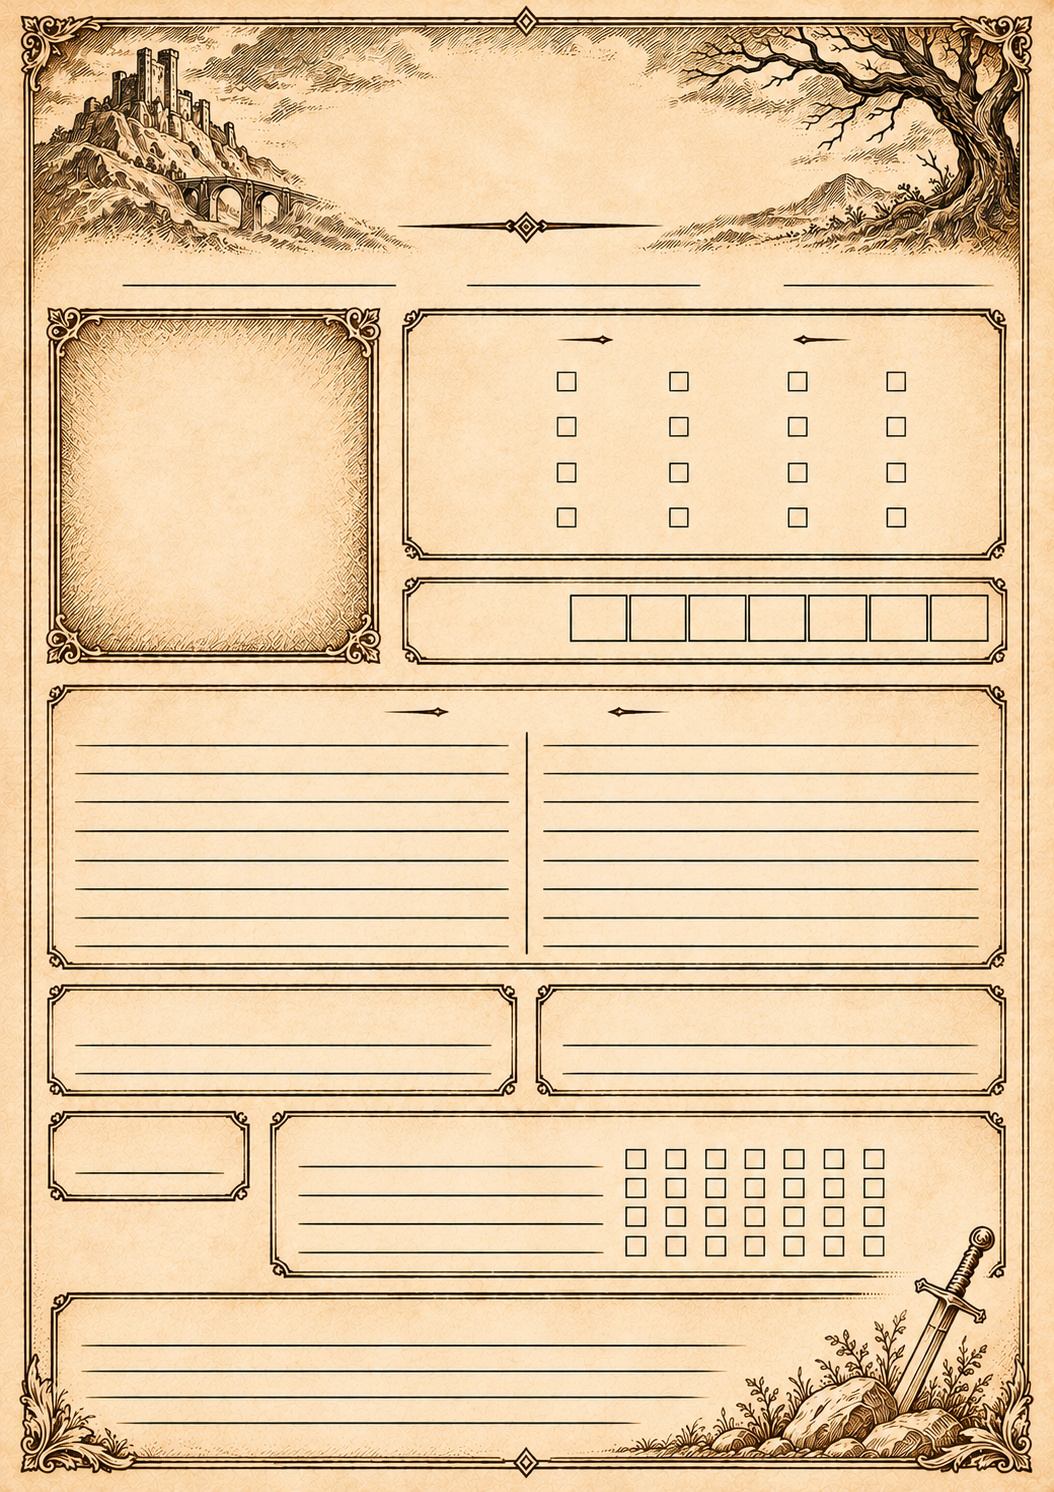
\includegraphics[width=210mm,height=297mm]{assets/character-background.jpg}}
\renewcommand\SheetArtwork{\xusebox{PregenArtwork}}
\fi
% Keys of one character. The Abilities columns (left, right) are lists of {paragraphs}; keep at
% least two items in a list whose text has commas, or the commas would split it. Trait, burden
% and notes are plain text.
\pgfkeys{/pregen/.is family,/pregen,
  name/.store in=\PregenName, race/.store in=\PregenRace, class/.store in=\PregenClass,
  portrait/.store in=\PregenPortrait,
  tiers/.store in=\PregenTiers,% tier of Strength, Dexterity, Lore, Wonder: 1 Untrained ... 4 Exceptional
  hp/.store in=\PregenHp,% maximum Hit Points; the boxes above it are shaded
  left/.store in=\PregenLeft, right/.store in=\PregenRight, weapon/.store in=\PregenWeapon,
  trait/.store in=\PregenTrait, burden/.store in=\PregenBurden,
  armour/.store in=\PregenArmour, armour tn/.store in=\PregenArmourTn,
  notes/.store in=\PregenNotes}
% build.sh builds one PDF per character: it defines \PregenOnly as that character's portrait key,
% and every other \PregenSheet call prints nothing.
\newcommand\PregenSheet[1]{%
  \pgfkeys{/pregen,name=,race=,class=,portrait=,tiers={1,1,1,1},hp=7,left=,right=,weapon=,trait=,burden=,
    armour=,armour tn=,notes=,#1}%
  \ifdefined\PregenOnly\ifx\PregenPortrait\PregenOnly\PregenPrint\fi\else\PregenPrint\fi}
\newcommand\PregenPrint{\let\SheetFill\PregenFill\SheetPage\clearpage}
% Free text after a label on the same baseline: starts 2.5 mm after the label (never before the
% engraved line starts) and shrinks only if it would run past the end of the line.
% #1 label x, #2 row y, #3 label text, #4 line start, #5 line end, #6 value
\newcommand\PregenAfterLabel[6]{%
  \pgfinterruptpicture\global\setbox\SheetMeasure\hbox{\RPGBodyBold\fontsize{10}{10}\selectfont#3}%
  \endpgfinterruptpicture
  \pgfmathsetmacro\PregenX{max(#4+1,#1+\wd\SheetMeasure*25.4/72.27+2.5)}%
  \pgfmathsetmacro\PregenW{#5-1-\PregenX}%
  \SheetFit{base west}{\PregenX}{#2}{\PregenFont{10.5}}{\PregenW}{#6}}
% A block of paragraphs written on ruled lines: #1 x, #2 y of the first engraved line, #3 font size,
% #4 width in mm, #5 line pitch in mm, #6 most lines allowed, #7 list of {paragraphs}.
% Wrapped lines of a paragraph are indented 3 mm; the build stops if the block needs more lines.
\newsavebox\PregenBlock
\newcommand\PregenRuled[7]{%
  \pgfinterruptpicture
  % No \color in here: a colour whatsit as first item would drop the \vtop's baseline to its top.
  \global\setbox\PregenBlock\vtop{\hsize=#4mm\PregenFont{#3}%
    \baselineskip=#5mm\lineskiplimit=-\maxdimen\parindent=0pt\parskip=0pt
    \rightskip=0pt plus 1fil\hyphenpenalty=10000\exhyphenpenalty=10000
    \foreach \PregenPar in #7 {\hangindent=3mm\hangafter=1\strut\PregenPar\strut\par}}%
  % n lines measure (n-1) pitches plus one strut (at most 3.5 mm up to 10 pt): allow half a pitch more.
  \pgfmathsetmacro\PregenMax{(#6-0.5)*#5+3.5}%
  \ifdim\dimexpr\ht\PregenBlock+\dp\PregenBlock\relax>\PregenMax mm\relax
    \PackageError{pregen-fill}{More than #6 lines in a ruled block on \PregenName's sheet}{}\fi
  \endpgfinterruptpicture
  \node[anchor=base west,inner sep=0pt,text=sheetink] at (#1,#2-1.3) {\usebox\PregenBlock};}
% One line of text on baseline y, shrunk only when wider than the free width:
% #1 x, #2 baseline y, #3 font size, #4 free width in mm, #5 text.
\newcommand\PregenLine[5]{%
  \pgfinterruptpicture\global\setbox\SheetMeasure\hbox{\PregenFont{#3}#5}%
  \ifdim\wd\SheetMeasure>#4mm\relax
    \global\setbox\SheetMeasure\hbox{\resizebox{#4mm}{!}{\box\SheetMeasure}}\fi
  \endpgfinterruptpicture
  \node[anchor=base west,inner sep=0pt,text=sheetink] at (#1,#2) {\usebox\SheetMeasure};}
% Tier mark: an X inside the 3.6 mm checkbox, 0.8 mm clear of its edges.
\def\PregenBoxX#1{\ifcase#1\or112.8\or135.2\or158.85\or178.5\fi}
\newcommand\PregenMark[2]{\draw[sheetink,line width=.9pt,line cap=round]
  (#1-1,#2-1)--(#1+1,#2+1) (#1-1,#2+1)--(#1+1,#2-1);}
% Hit-point boxes, measured on the artwork: inner left and right edges in mm; inside, the boxes
% run from 118.7 to 127.3 mm.
\def\PregenHpL#1{\ifcase#1\or114.0\or125.7\or137.5\or149.4\or161.4\or173.5\or185.7\fi}
\def\PregenHpR#1{\ifcase#1\or124.7\or136.5\or148.4\or160.2\or172.5\or184.5\or196.7\fi}
% Notes: three engraved lines at 267.8, 272.9 and 278.1 mm, ending at 145.1, 142.3 and 138.9 mm.
% The first runs under the NOTES label, so the text starts 2.5 mm after the label; the build
% stops if the notes need a fourth line.
\newcommand\PregenNotesBlock{%
  \pgfinterruptpicture
  \global\setbox\SheetMeasure\hbox{\RPGBodyBold\fontsize{10}{10}\selectfont\Sh{Notes}\SheetColon}%
  \pgfmathsetmacro\PregenIndent{15+\wd\SheetMeasure*25.4/72.27+2.5-19}%
  \global\setbox\PregenBlock\vtop{\PregenFont{8.5}\baselineskip=5.15mm\lineskiplimit=-\maxdimen
    \parindent=0pt\parskip=0pt\rightskip=0pt plus 1fil\hyphenpenalty=10000\exhyphenpenalty=10000
    \parshape 3 \PregenIndent mm \dimexpr125mm-\PregenIndent mm\relax 0mm 122.3mm 0mm 118.9mm
    \strut\PregenNotes\strut\par}%
  \ifdim\dimexpr\ht\PregenBlock+\dp\PregenBlock\relax>16.4mm\relax
    \PackageError{pregen-fill}{More than three lines of notes on \PregenName's sheet}{}\fi
  \endpgfinterruptpicture
  \node[anchor=base west,inner sep=0pt,text=sheetink] at (19,266.5) {\usebox\PregenBlock};}
\newcommand\PregenFill{%
  % Portrait: inside the frame's inner edge (12.2--72.5 x 64.4--129.5 mm), clear of its hatching.
  \ifdefined\SheetTextOnly\else
  \node[anchor=south,inner sep=0pt] at (42.35,127.6)
    {\includegraphics[width=55mm,height=60mm,keepaspectratio]{../assets/hollow-hearth/pregens/\PregenPortrait.png}};
  \fi
  % Identity: on the label's baseline, over the engraved lines at 56.8 mm.
  \PregenAfterLabel{13}{52.5}{\Sh{Name}\SheetColon}{24.5}{78.7}{\PregenName}
  \PregenAfterLabel{82}{52.5}{\Sh{Race}\SheetColon}{93}{139.3}{\PregenRace}
  \PregenAfterLabel{151}{52.5}{\Sh{Class}\SheetColon}{156.2}{196.5}{\PregenClass}
  % One tier per attribute (rows at 76, 85.2, 94.3, 103.6 mm; boxes centred 0.1 mm higher).
  \foreach \PregenT [count=\PregenRow] in \PregenTiers {%
    \pgfmathsetmacro\PregenY{{76,85.2,94.3,103.6}[\PregenRow-1]-0.1}%
    \PregenMark{\PregenBoxX{\PregenT}}{\PregenY}}
  % Boxes above the maximum are shaded (a cross would read as a wound); the others stay free.
  % The maximum is written under the HIT POINTS label (free from 84 to 112 mm down to 130.8 mm).
  \foreach \PregenN in {1,...,7} {\ifnum\PregenN>\PregenHp\relax
    \fill[sheetink,opacity=.2] (\PregenHpL{\PregenN}+.3,119) rectangle (\PregenHpR{\PregenN}-.3,127);\fi}
  \PregenLine{84}{129.4}{7.5}{27}{\Sh{HpMax}{\PregenHp}}
  % Abilities: eight engraved lines per column, 148.4--188.4 mm (5.714 mm pitch). The right
  % column starts on its second line: its first one runs under the ABILITIES heading. The weapon
  % has its own labelled field on the last line of the left column, apart from the skills.
  \PregenRuled{16.5}{148.4}{9}{83}{5.714}{7}{\PregenLeft}
  \ifx\PregenWeapon\empty\else
    \PregenLine{16.5}{187.1}{9}{83}{\Sh{Weapon}\SheetColon\enspace\PregenWeapon}\fi
  \ifx\PregenRight\empty\else\PregenRuled{109.8}{154.114}{8.6}{83.5}{5.714}{7}{\PregenRight}\fi
  % Trait and Burden: two engraved lines each, at 208.2 and 213.8 mm.
  \PregenRuled{16.5}{208.2}{9.5}{79.5}{5.6}{2}{{\PregenTrait}}
  \PregenRuled{113.6}{208.2}{9.5}{79.5}{5.6}{2}{{\PregenBurden}}
  % Armour: its name on the engraved line (15.1--44.4 mm at 233.6 mm), the TNs below it,
  % above the frame's bottom rule at 238.1 mm.
  \PregenLine{16.2}{232.3}{9.5}{27.5}{\PregenArmour}
  \PregenLine{16.2}{236.6}{7.5}{27.5}{\PregenArmourTn}
  \PregenNotesBlock}
